\documentclass[12pt,a4paper]{article}

% ─── Page Layout ───────────────────────────────────────────────────────────────
\usepackage[a4paper, margin=0.8in, headheight=14pt]{geometry}

% ─── Fonts (XeLaTeX) ───────────────────────────────────────────────────────────
\usepackage{fontspec}
\usepackage{unicode-math}
\setmainfont{TeX Gyre Pagella}
\setmonofont[Scale=0.88]{TeX Gyre Cursor}
\setmathfont{Latin Modern Math}

% ─── Packages ──────────────────────────────────────────────────────────────────
\usepackage{xcolor}
\usepackage{colortbl}
\usepackage{titlesec}
\usepackage{enumitem}
\usepackage{tabularx}
\usepackage{booktabs}
\usepackage{array}
\usepackage{amsmath}
\usepackage{tikz}
\usetikzlibrary{shapes.geometric, arrows.meta, positioning, calc, fit, decorations.pathreplacing}
\usepackage{tcolorbox}
\tcbuselibrary{skins, breakable}
\usepackage{hyperref}
\usepackage{fancyhdr}
\usepackage{graphicx}
\usepackage{microtype}
\hyphenpenalty=10000
\exhyphenpenalty=10000
\sloppy
\usepackage{caption}
\usepackage{setspace}
\usepackage{multirow}
\usepackage{tocloft}

% ─── Q&A helper ────────────────────────────────────────────────────────────────
\newcommand{\Q}[1]{\textbf{#1}\par\noindent\ignorespaces}

% ─── Colour Palette ────────────────────────────────────────────────────────────
\definecolor{myred}{RGB}{196,30,58}
\definecolor{mydark}{RGB}{30,30,50}
\definecolor{mygreen}{RGB}{14,120,80}
\definecolor{myteal}{RGB}{0,130,140}
\definecolor{myamber}{RGB}{180,100,0}
\definecolor{mypurple}{RGB}{100,30,160}
\definecolor{mygray}{RGB}{246,247,249}
\definecolor{mgframe}{RGB}{180,185,200}
\definecolor{watermark}{RGB}{145,150,170}
\definecolor{hdrred}{RGB}{250,232,235}
\definecolor{hdrgreen}{RGB}{220,244,233}
\definecolor{hdrteal}{RGB}{220,242,244}
\definecolor{hdramber}{RGB}{253,242,215}
\definecolor{hdrpurple}{RGB}{238,228,255}
\definecolor{hdrgray}{RGB}{238,240,245}
\definecolor{rowalt}{RGB}{250,251,253}

% ─── Section Formatting ────────────────────────────────────────────────────────
\titleformat{\section}
  {\large\bfseries\color{myred}}{\thesection.}{0.5em}{}
  [\vspace{1pt}{\color{myred}\rule{\linewidth}{0.8pt}}]
\titleformat{\subsection}
  {\normalsize\bfseries\color{myteal}}{\thesubsection}{0.5em}{}
\titlespacing*{\section}{0pt}{18pt}{7pt}
\titlespacing*{\subsection}{0pt}{11pt}{4pt}

% ─── Paragraph ─────────────────────────────────────────────────────────────────
\setlength{\parindent}{0pt}
\setlength{\parskip}{4pt}

% ─── TOC Styling ───────────────────────────────────────────────────────────────
\renewcommand{\cfttoctitlefont}{\large\bfseries\color{myred}}
\renewcommand{\cftaftertoctitle}{\par\noindent{\color{myred}\rule{\linewidth}{0.8pt}}}
\setlength{\cftbeforetoctitleskip}{0pt}
\setlength{\cftaftertoctitleskip}{6pt}
\renewcommand{\cftsecfont}{\normalsize\bfseries\color{mydark}}
\renewcommand{\cftsecpagefont}{\normalsize\bfseries\color{mydark}}
\renewcommand{\cftsecleader}{\cftdotfill{\cftdotsep}}
\setlength{\cftbeforesecskip}{7pt}
\renewcommand{\cftsubsecfont}{\small\color{mydark}}
\renewcommand{\cftsubsecpagefont}{\small\color{mydark}}
\setlength{\cftbeforesubsecskip}{3pt}
\setlength{\cftsubsecindent}{1.4em}

% ─── Table helpers ─────────────────────────────────────────────────────────────
\renewcommand{\arraystretch}{1.45}
\setlength{\tabcolsep}{6pt}
\arrayrulecolor{mydark}
\newcolumntype{B}[1]{>{\small\bfseries\raggedright\arraybackslash}m{#1}}
\newcolumntype{Y}{>{\small\raggedright\arraybackslash}X}
\renewcommand{\tabularxcolumn}[1]{m{#1}}

% ─── Header / Footer ───────────────────────────────────────────────────────────
\pagestyle{fancy}
\fancyhf{}
\fancyhead[L]{\small\color{myred}\textbf{OE-EC604C}\;\color{mydark}--- Object Oriented Programming}
\fancyhead[R]{\small\color{myteal}\textbf{Module 9 Notes}}
\fancyfoot[C]{\small\color{mydark}\thepage}
\fancyfoot[R]{\small\color{watermark}\textit{\copyright\ Biraj}}
\renewcommand{\headrulewidth}{0.5pt}
\renewcommand{\footrulewidth}{0.3pt}

% ─── Hyperref ──────────────────────────────────────────────────────────────────
\hypersetup{
  colorlinks=true, linkcolor=myteal, urlcolor=myteal,
  pdfauthor={Biraj Sarkar},
  pdftitle={OE-EC604C --- Module 9 Notes}
}

% ─── tcolorbox styles ──────────────────────────────────────────────────────────
\tcbset{
  tikzbox/.style={
    colback=mygray, colframe=mgframe, boxrule=0.6pt, arc=4pt,
    left=8pt, right=8pt, top=6pt, bottom=6pt,
    colbacktitle=mgframe, coltitle=mydark,
    fonttitle=\small\bfseries
  },
  defbox/.style={
    colback=hdrgreen, colframe=mygreen, boxrule=0.8pt, arc=4pt,
    left=9pt, right=9pt, top=6pt, bottom=6pt,
    colbacktitle=mygreen, coltitle=white,
    fonttitle=\small\bfseries
  },
  formulabox/.style={
    colback=hdrteal, colframe=myteal, boxrule=0.8pt, arc=4pt,
    left=9pt, right=9pt, top=7pt, bottom=7pt,
    colbacktitle=myteal, coltitle=white,
    fonttitle=\small\bfseries
  },
  examplebox/.style={
    colback=hdramber, colframe=myamber, boxrule=0.8pt, arc=4pt,
    left=9pt, right=9pt, top=6pt, bottom=6pt,
    colbacktitle=myamber, coltitle=white,
    fonttitle=\small\bfseries
  },
  masonbox/.style={
    colback=hdrpurple, colframe=mypurple, boxrule=0.8pt, arc=4pt,
    left=9pt, right=9pt, top=6pt, bottom=6pt,
    colbacktitle=mypurple, coltitle=white,
    fonttitle=\small\bfseries
  },
  exambox/.style={
    colback=hdrpurple, colframe=mypurple, boxrule=1pt, arc=5pt,
    left=10pt, right=10pt, top=8pt, bottom=8pt,
    colbacktitle=mypurple, coltitle=white,
    fonttitle=\bfseries,
    breakable, title after break={\textbf{Frequently Asked / Viva Questions (contd.)}}}
}

% XeLaTeX pdfcol fix: reset text color after every tcolorbox
\tcbset{after={\color{black}}}

% ─── TikZ styles ───────────────────────────────────────────────────────────────
\tikzset{
  block/.style={rectangle, draw=myteal, fill=hdrteal,
    text width=2.4cm, align=center, minimum height=0.95cm,
    font=\small, rounded corners=3pt, line width=0.7pt},
  redblock/.style={rectangle, draw=myred, fill=hdrred,
    text width=2.4cm, align=center, minimum height=0.95cm,
    font=\small, rounded corners=3pt, line width=0.7pt},
  netnode/.style={rectangle, draw=myteal, fill=hdrteal,
    text width=1.5cm, align=center, minimum height=0.8cm,
    font=\small, rounded corners=3pt, line width=0.7pt},
  sumjunc/.style={circle, draw=myamber, fill=hdramber,
    minimum size=0.62cm, font=\small, line width=0.8pt},
  snode/.style={circle, draw=mypurple, fill=hdrpurple,
    minimum size=0.55cm, font=\footnotesize, line width=0.7pt},
  arrow/.style={-Stealth, thick, color=mydark},
  redarrow/.style={-Stealth, thick, color=myred},
  line/.style={thick, color=mydark}
}

% ═══════════════════════════════════════════════════════════════════════════════
\begin{document}
% ═══════════════════════════════════════════════════════════════════════════════

\begin{center}
  {\LARGE\bfseries\color{myred} OE-EC604C --- Object Oriented Programming}\\[5pt]
  {\normalsize\color{mydark} Semester VI \quad$\bullet$\quad 3L:0T:0P \quad$\bullet$\quad 3 Credits}\\[3pt]
  {\normalsize\color{myteal}\textbf{Module 9 Exam Notes: Exception Handling \& Templates}}\\[3pt]
  {\small\color{mydark} CGEC \;$|$\; B.Tech ECE (2023--27) \;$|$\; \textit{Biraj Sarkar}}
\end{center}
\vspace{2pt}
\noindent{\color{myred}\rule{\linewidth}{1.5pt}}
\vspace{2pt}

\hypersetup{linkcolor=mydark}
\tableofcontents
\hypersetup{linkcolor=myteal}
\newpage

% ===============================================================================
\section{Exception Handling Mechanism}
% ===============================================================================

Exception handling separates error detection from error resolution, allowing applications to recover gracefully from runtime errors.

\subsection{Basic Syntax: \texorpdfstring{\texttt{try}}{try}, \texorpdfstring{\texttt{throw}}{throw}, and \texorpdfstring{\texttt{catch}}{catch}}
\begin{itemize}[leftmargin=*, itemsep=3.5pt]
  \item \textbf{\texttt{try} block:} Encloses the segment of code where exceptions might occur.
  \item \textbf{\texttt{throw} statement:} Triggers an exception when an anomaly is detected, exiting the try block immediately.
  \item \textbf{\texttt{catch} block:} Defines a handler that matches the data type of the thrown exception to resolve the error.
\end{itemize}

\subsection{Exception Propagation \& Stack Unwinding}
If a throw point occurs inside a nested function, the compiler exits that function immediately. It searches up the function call stack for an active \texttt{try} block.
During this process, the compiler invokes destructors for all local variables created inside the exited stack frames. This process is called \textbf{Stack Unwinding}.

\begin{tcolorbox}[tikzbox, title={Exception Handling Control Flow Map}]
\centering
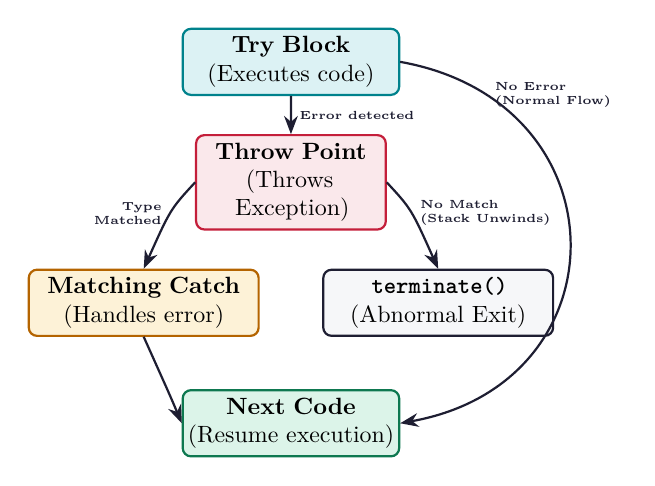
\begin{tikzpicture}[node distance=1.5cm, thick, scale=0.85, every node/.style={scale=0.85}]
  % Blocks
  \node[rectangle, draw=myteal, fill=hdrteal, rounded corners=3pt, text width=3.0cm, align=center, minimum height=0.8cm] (try) at (0, 2.4) {\textbf{Try Block} \\ (Executes code)};
  
  \node[rectangle, draw=myred, fill=hdrred, rounded corners=3pt, text width=2.6cm, align=center, minimum height=0.8cm] (throw) at (0, 0.6) {\textbf{Throw Point} \\ (Throws Exception)};
  
  \node[rectangle, draw=myamber, fill=hdramber, rounded corners=3pt, text width=3.2cm, align=center, minimum height=0.8cm] (catch) at (-2.2, -1.2) {\textbf{Matching Catch} \\ (Handles error)};
  
  \node[rectangle, draw=mydark, fill=mygray, rounded corners=3pt, text width=3.2cm, align=center, minimum height=0.8cm] (terminate) at (2.2, -1.2) {\textbf{\texttt{terminate()}} \\ (Abnormal Exit)};

  \node[rectangle, draw=mygreen, fill=hdrgreen, rounded corners=3pt, text width=3.0cm, align=center, minimum height=0.8cm] (next) at (0, -3.0) {\textbf{Next Code} \\ (Resume execution)};

  % Flows
  \draw[arrow] (try) -- (throw) node[midway, right, font=\tiny\bfseries\color{myred}] {Error detected};
  
  \draw[arrow] (throw.west) .. controls (-1.8, 0.2) .. (catch.north) node[midway, left, font=\tiny\bfseries\color{myteal}, align=right] {Type\\Matched};
  
  \draw[arrow] (throw.east) .. controls (1.8, 0.2) .. (terminate.north) node[midway, right, font=\tiny\bfseries\color{myamber}, align=left] {No Match\\(Stack Unwinds)};
  
  \draw[arrow] (catch.south) .. controls (-1.8, -2.6) .. (next.west);
  
  \draw[arrow] (try.east) .. controls (5.0, 1.8) and (5.0, -2.4) .. (next.east) node[pos=0.15, right, font=\tiny\bfseries\color{mygreen}, align=left] {No Error\\(Normal Flow)};
\end{tikzpicture}
\end{tcolorbox}

\begin{tcolorbox}[examplebox, title={Code Example: Exception throw point outside the main try block}]
\begin{spacing}{1.0}
\begin{verbatim}
#include <iostream>
// Function that throws exception
double divide(double a, double b) {
    if(b == 0.0) {
        throw "Division by zero condition!"; // Throws a const char*
    }
    return a / b;
}

int main() {
    double x = 10, y = 0, result;
    try {
        result = divide(x, y); // Throw point is inside divide()
        std::cout << "Result = " << result << std::endl;
    }
    catch(const char* msg) { // Catches the thrown char*
        std::cerr << "Caught Exception: " << msg << std::endl;
    }
    return 0;
}
\end{verbatim}
\end{spacing}
\end{tcolorbox}

\subsection{Multiple Catches, Catch-All, and Re-throwing}
\begin{itemize}[leftmargin=*, itemsep=3pt]
  \item \textbf{Multiple Catches:} A single try block can have multiple sequential catch handlers to process different exception types.
  \item \textbf{Catch-All (\texttt{catch(...)}):} A special catch handler that intercepts any exception type. It must be placed at the very end of the handler list.
  \item \textbf{Exception Re-throwing:} An caught exception can be re-thrown using the \texttt{throw;} statement without arguments inside the catch block to pass it up to a higher scope.
\end{itemize}

% ===============================================================================
\section{Generic Programming using Templates}
% ===============================================================================

Templates allow writing code that is independent of data types, enabling the creation of generic functions and classes.

\subsection{Function Templates}
Function templates act as formulas for generating functions based on argument types.
\begin{tcolorbox}[formulabox, title={\textbf{Function Template Syntax}}]
\begin{equation}
  \texttt{template <typename T> } \quad \text{Return\_Type} \quad \text{FuncName}(\text{T args}) \quad \{ \dots \}
\end{equation}
\end{tcolorbox}

\begin{tcolorbox}[examplebox, title={Code Example: Multi-parameter function template}]
\begin{spacing}{1.0}
\begin{verbatim}
#include <iostream>
// Multi-parameter function template
template <typename T1, typename T2>
void printComparison(T1 x, T2 y) {
    if(x > y) {
        std::cout << x << " is larger than " << y << std::endl;
    } else {
        std::cout << x << " is not larger than " << y << std::endl;
    }
}

int main() {
    printComparison(10, 5.5); // T1 = int, T2 = double
    printComparison(4.2, 9.8); // T1 = double, T2 = double
    return 0;
}
\end{verbatim}
\end{spacing}
\end{tcolorbox}

\subsection{Class Templates}
Class templates are used to create generic containers or data structures that operate on any data type.
\begin{tcolorbox}[examplebox, title={Code Example: Generic Stack class template}]
\begin{spacing}{1.0}
\begin{verbatim}
#include <iostream>
template <typename T, int SIZE = 10> // typename T and non-type int SIZE
class Stack {
private:
    T arr[SIZE];
    int top;
public:
    Stack() : top(-1) {}
    
    bool push(T element) {
        if(top >= SIZE - 1) return false; // Overflow
        arr[++top] = element;
        return true;
    }
    
    T pop() {
        if(top < 0) throw "Stack Underflow!"; // Throw const char*
        return arr[top--];
    }
};

int main() {
    try {
        Stack<int, 5> intStack; // Instantiate an int stack of size 5
        intStack.push(10);
        intStack.push(20);
        std::cout << intStack.pop() << std::endl; // 20
        std::cout << intStack.pop() << std::endl; // 10
        std::cout << intStack.pop() << std::endl; // Throws exception
    }
    catch(const char* e) {
        std::cout << "Exception: " << e << std::endl;
    }
    return 0;
}
\end{verbatim}
\end{spacing}
\end{tcolorbox}

% ===============================================================================
% MANDATORY QUICK REVISION PAGE
% ===============================================================================
\newpage
\begin{center}
  {\large\bfseries\color{myred} Quick Revision --- Module IX}\\[3pt]
  {\small\color{mydark} Exception Handling \& Templates $|$ OE-EC604C}
\end{center}
\noindent{\color{myred}\rule{\linewidth}{1.2pt}}
\vspace{4pt}

\begin{tcolorbox}[formulabox, title={\textbf{Key Exception and Template Syntax}}]
\renewcommand{\arraystretch}{1.3}
\begin{tabularx}{\linewidth}{B{3.8cm} X}
Try-Catch Block          & \texttt{try \{ throw 404; \} catch(int err) \{ /* handles 404 */ \}} \\[4pt]
Catch-All Handler        & \texttt{catch(...) \{ /* catches any exception type */ \}} \\[4pt]
Re-throwing              & \texttt{catch(const char* e) \{ throw; // Re-throws exception up \} } \\[4pt]
Function Template        & \texttt{template <typename T> T maxVal(T a, T b) \{ return (a > b) ? a : b; \}} \\[4pt]
Class Template           & \texttt{template <class T> class Box \{ T value; \};} \\[4pt]
Template Instantiation   & \texttt{Box<double> doubleBox; // Explicit template argument}
\end{tabularx}
\end{tcolorbox}

\begin{tcolorbox}[defbox, title={\textbf{One-Line Definitions}}]
\begin{itemize}[leftmargin=*, itemsep=2.5pt, topsep=0pt]
  \item \textbf{Exception:} A runtime error or anomaly that disrupts the normal execution flow of a program.
  \item \textbf{Stack Unwinding:} The automatic destruction of local variables in stack frames during exception propagation.
  \item \textbf{Catch-All Handler:} A fallback handler (\texttt{catch(...)}) that catches any exception type not previously intercepted.
  \item \textbf{Re-throwing:} Forwarding an caught exception up to the parent calling frame using the \texttt{throw;} statement.
  \item \textbf{Template:} A blueprint used by the compiler to generate type-specific functions or classes automatically.
  \item \textbf{Generic Programming:} A programming model focused on writing algorithms independent of specific data types.
  \item \textbf{Non-type Template Parameter:} A template parameter that represents a constant value (e.g., \texttt{int SIZE}) rather than a type.
  \item \textbf{Template Specialization:} Defining a unique template implementation for a specific data type (e.g., \texttt{T = char*}).
  \item \textbf{terminate():} A system function called when no matching catch handler is found for a thrown exception.
\end{itemize}
\end{tcolorbox}

\begin{tcolorbox}[exambox, title={\textbf{Frequently Asked / Viva Questions}}]
\begin{enumerate}[topsep=0pt, label=\textbf{Q\arabic*.}, itemsep=5pt]
  \item \Q{What happens if an exception is thrown but no matching catch block is found?}
    The runtime library calls the \texttt{terminate()} function, which by default calls \texttt{abort()} to terminate the program immediately.
  \item \Q{Can we throw class objects as exceptions in C++?}
    Yes. Throwing class instances is the standard way to implement custom exceptions, allowing structured error data to be passed to handlers.
  \item \Q{What is the purpose of the catch-all handler and where must it be placed?}
    \texttt{catch(...)} catches all exception types. It acts as a safety net and must be placed as the last handler, otherwise it blocks subsequent handlers.
  \item \Q{Why does template instantiation not happen at class definition time?}
    A template only defines a blueprint. The compiler only generates class code when the template is instantiated with a specific type (e.g., \texttt{Stack<int>}).
  \item \Q{Explain the compile-time overhead associated with templates.}
    Templates require the compiler to generate unique code for each type instantiation, which increases compile times and binary sizes (code bloat).
  \item \Q{What is template function specialization?}
    It allows defining a custom implementation of a function template for a specific data type (e.g., optimizing string comparisons instead of pointer comparisons).
  \item \Q{Can templates have default arguments?}
    Yes. Both class templates and function templates (in C++11) can have default type arguments (e.g., \texttt{template <typename T = int>}).
  \item \Q{How does the compiler select between overloaded template functions and regular functions?}
    The compiler prefers a regular non-template function if it matches the arguments exactly. If no match is found, it instantiates the template.
  \item \Q{Explain the difference between exception handling in C++ vs. Java.}
    C++ does not support checked exceptions (you do not have to declare exceptions in method signatures), and it does not have a native \texttt{finally} block (resource cleanup relies on RAII).
  \item \Q{What is the difference between \texttt{typename} and \texttt{class} keywords in template declarations?}
    Inside template parameters, \texttt{typename} and \texttt{class} are completely equivalent and interchangeable. E.g., \texttt{template <class T>} and \texttt{template <typename T>} behave identically.
  \item \Q{Why is it dangerous to throw pointers to local variables?}
    Local variables are destroyed when stack frames are unwound. The handler will receive a dangling pointer to invalid memory, causing undefined behavior.
  \item \Q{What is the RAII (Resource Acquisition Is Initialization) pattern?}
    It is a design pattern where resources (files, memory, locks) are bound to the lifetime of local objects. Destructors automatically release resources during normal exit or stack unwinding, preventing leaks.
\end{enumerate}
\end{tcolorbox}

\begin{tcolorbox}[tikzbox, title={Comparison: Exception Handling vs. Traditional Error Return Codes}]
\renewcommand{\arraystretch}{1.45}
\par\noindent
\begin{tabularx}{\linewidth}{|B{3.2cm}|Y|Y|}
\hline
\textbf{Feature} & \textbf{\color{myteal}Exception Handling (try-catch)} & \textbf{\color{myamber}Traditional Error Codes (if-else)} \\
\hline
\textbf{Separation} & Clear separation between execution logic and error handling code. & Error checking logic is mixed directly into the main algorithm. \\
\hline
\textbf{Propagation} & Errors propagate automatically up the call stack until handled. & Errors must be explicitly returned and checked in every function frame. \\
\hline
\textbf{Data Payload} & Exceptions can pass complex objects containing detailed error info. & Limited to returning simple integer codes or status booleans. \\
\hline
\textbf{Performance} & Slower when exceptions occur (due to stack unwinding and V-Table lookup). & Minimal overhead (simple conditional branches). \\
\hline
\textbf{Uncaught Errors} & Leads to immediate program termination (safe fail-fast). & Can be silently ignored, causing latent bugs or data corruption. \\
\hline
\end{tabularx}
\end{tcolorbox}

\end{document}
